%% LyX 2.3.6.1 created this file.  For more info, see http://www.lyx.org/.
%% Do not edit unless you really know what you are doing.
\documentclass[english]{article}
\usepackage[T1]{fontenc}
\usepackage[latin9]{inputenc}
\usepackage{geometry}
\geometry{verbose,tmargin=2.5cm,bmargin=2.5cm,lmargin=2.5cm,rmargin=2.5cm}
\usepackage{calc}
\usepackage{graphicx}

\makeatletter

%%%%%%%%%%%%%%%%%%%%%%%%%%%%%% LyX specific LaTeX commands.
%% Because html converters don't know tabularnewline
\providecommand{\tabularnewline}{\\}

\makeatother

\usepackage{babel}
\begin{document}
{[}SPLIT\_HERE{]}
\begin{enumerate}
\item \textbf{{[}PJC/PRELIM/9597/2014/P2/Q1{]} }

A manual system for producing school student reports works in the
following manner: 
\begin{itemize}
\item a subject report is completed for each subject that a student takes
by the single teacher teaching that subject; 
\item to help the subject teacher, initially a blank report form is issued
to the student for the student to add their details: student NRIC,
name, contact phone, teacher and class; 
\item the subject report is completed by the teacher with appropriate comments; 
\item all subject reports for the student are passed to the student's tutor; 
\item the tutor puts all the subject reports together to form the student's
report folder; 
\item the tutor adds a tutor's report including attendance data supplied
by the school administration attendance records; 
\item each student's report folder is copied; 
\item the copy is filed in the report storage facility for the school; 
\item the report folder is sent to the student's parents. 
\end{itemize}
The school has decided to replace this manual system with a computerised
system. 

A system developer is employed to carry out the task. The first task
assigned to the system developer is to write a project proposal.
\begin{enumerate}
\item One section of the project proposal is the Problem Statement which
lists the problems in the current system. Write the Problem Statement.\hfill{}
{[}4{]}
\item The proposal is accepted and the main stages of the project have been
identified and durations assessed as follows: 

\begin{tabular}{|c|l|c|l|}
\hline 
Stage & Description & Weeks & Staffing\tabularnewline
\hline 
\hline 
A & analysis of the solution & 4 & Analyst A1\tabularnewline
\hline 
B & design of the solution & 8 & Analysts A2 and A3 \tabularnewline
\hline 
C & development of the solution & 12 & Programmers P1 and P2\tabularnewline
\hline 
D & documentation of the solution & 8 & Clerks C1 and C2\tabularnewline
\hline 
E & implementation of the solution & 6 & Programmer P1\tabularnewline
\hline 
F & testing of the solution & 4 & Programmers P3 and P4\tabularnewline
\hline 
\end{tabular}

B and D cannot start until A is completed 

F and C cannot start until B is completed 

E cannot start until C is completed 

The project will end when D, E and F are completed.
\begin{enumerate}
\item Draw a Program Evaluation and Review Technique (PERT) chart for these
6 project stages (A to F). \hfill{}{[}4{]}
\item Calculate and display on the diagram, with a node layout key, the
earliest and latest start and finish times of each task. \hfill{}{[}4{]}
\item State the critical path.\hfill{} {[}1{]}
\item State the minimum time in which the project could be completed. \hfill{}{[}1{]}
\item Explain dependent stages and concurrent stages. For each type of stage
give an example from this chart. \hfill{}{[}4{]}
\item A decision is made that the PERT chart should show more detail with
regard to testing. It is proposed that stage F (testing) should be
removed from the chart and three new stages added:

L -- black box testing -- 2 weeks 

M -- white box testing -- 2 weeks

N -- beta testing -- 3 weeks 

Redraw the PERT chart to show the effect of these changes.\hfill{}
{[}2{]}
\item Draw a Gantt chart showing all \textbf{eight} stages and their dependencies,
allowing for the resource allocations as indicated above. \hfill{}{[}4{]}
\item List and explain briefly \textbf{TWO} advantages and \textbf{ONE}
disadvantage of using a Program Evaluation and Review Technique (PERT)
chart for a project plan in comparison with using a Gantt chart. \hfill{}{[}3{]}
\end{enumerate}
\item Identify \textbf{FIVE} key stages with brief description of the software
development life cycle (SDLC). \hfill{}{[}3{]}
\item At which stage of the SDLC is top-down analysis used? Explains why
it helps in the solution of complex problems. \hfill{}{[}2{]}
\item The attendance data enter into the new system needs to be validated
and verified. Explain with examples the difference between data validation
and data verification. \hfill{}{[}4{]}
\item Marek is designing a program for this computerised system. His test
strategy includes beta testing and acceptance testing.
\begin{enumerate}
\item Describe what is meant by beta testing and how it can be used to test
Marek\textquoteright s program. \hfill{} {[}2{]}
\item Describe what is meant by acceptance testing and how it can be used
to test Marek\textquoteright s program. \hfill{}{[}2{]}
\end{enumerate}
\item Teachers spend part of their week working from home. A system analyst
will assist in improving their school communication systems. Explain
why it is important to define problem accurately. {[}2{]} 
\item Subject teachers and tutors are worried because so much information
is being stored about their students on the server of the school.
Describe the fears that the teachers may have and explain what the
school can do to allay those fears. \hfill{}{[}3{]}
\item When data is transmitted between devices on a network it is liable
to corruption. One way of checking data for corruption is to carry
out a check sum. What is check sum? \hfill{}{[}1{]}
\item Explain another method of checking data to ensure that it has been
transmitted without corruption. \hfill{}{[}2{]}
\item When data is transmitted on a network it can use a number of different
transmission modes. State what is meant by each of the following modes
of data transmission.
\begin{enumerate}
\item Simplex \hfill{}{[}1{]}
\item Duplex \hfill{}{[}1{]}
\item Half-duplex \hfill{} {[}1{]}
\end{enumerate}
\end{enumerate}
{[}SPLIT\_HERE{]}
\item \textbf{{[}PJC/PRELIM/9597/2014/P2/Q2{]} }

A programmer is going to write part of the computer system, using
an object-oriented programming language, which will store details
subject teachers and tutors. All teachers and tutors will be identified
by their NRICs. 

Properties identified the subject teachers: 
\begin{itemize}
\item Subject code 
\end{itemize}
Properties identified the tutors: 
\begin{itemize}
\item Class name 
\end{itemize}
\begin{enumerate}
\item Draw a diagram that shows how the properties could be distributed
amongst a number of classes. Include in your diagram any inheritance
between classes. Also indicate some of the methods that would be required.
\hfill{}{[}4{]}
\item In the context of object-oriented programming explain what is meant
by:
\begin{enumerate}
\item encapsulation; \hfill{}{[}1{]}
\item inheritance;\hfill{} {[}1{]}
\item polymorphism. \hfill{}{[}1{]}
\end{enumerate}
\item Give two advantages of object-oriented programming. \hfill{}{[}2{]}
\end{enumerate}
{[}SPLIT\_HERE{]}
\item \textbf{{[}PJC/PRELIM/9597/2014/P2/Q3{]} }

The words COW, BEEF and FORTY have all their letters written in alphabetical
order. Here is an algorithm for a function which checks whether all
the letters in a word are in alphabetical order. 

\noindent\begin{minipage}[t]{1\columnwidth}%
\texttt{01 FUNCTION IsInOrder(Word) }

\texttt{02 \qquad{}IF LENGTH(Word) = 1 THEN }

\texttt{03 \qquad{}\qquad{}RETURN TRUE }

\texttt{04 \qquad{}ELSE }

\texttt{05 \qquad{}\qquad{}FirstChar = First character in Word }

\texttt{06 \qquad{}\qquad{}RestOfWord = All characters in Word except
the first }

\texttt{07 \qquad{}\qquad{}IF FirstChar > RestOfWord THEN }

\texttt{08 \qquad{}\qquad{}\qquad{}RETURN FALSE }

\texttt{09 \qquad{}\qquad{}ELSE }

\texttt{10 \qquad{}\qquad{}\qquad{}RETURN IsInOrder(RestOfWord) }

\texttt{11 \qquad{}\qquad{}END IF }

\texttt{12 \qquad{}END IF }

\texttt{13 END FUNCTION} %
\end{minipage}
\begin{enumerate}
\item State what is meant by recursion using this algorithm as an example.
\hfill{}{[}2{]}
\item The algorithm is tested with the call \texttt{IsInOrder(\textquotedbl Z\textquotedbl )}.
State the value which will be returned. State the lines of the algorithm
which will be executed. \hfill{}{[}2{]}
\item Explain what happens if the algorithm is tested with a call \texttt{IsInOrder(\textquotedbl{}
\textquotedbl )} where the value of the argument is the empty string.
\hfill{}{[}2{]}
\item Explain what happens when the algorithm is tested with the call \texttt{IsInOrder(\textquotedbl APE\textquotedbl )}.
You should show each call made, the lines of the algorithm executed
and the return value of each call. You may use a diagram.\hfill{}
{[}4{]}
\end{enumerate}
{[}SPLIT\_HERE{]}
\item \textbf{{[}PJC/PRELIM/9597/2014/P2/Q4{]} }

Character sets are used in computers to perform tasks. 
\begin{enumerate}
\item Explain how a character set is used by a computer. \hfill{}{[}2{]}
\item Explain the differences between Unicode and ASCII.\hfill{} {[}2{]}
\item The ASCII representation for character A is 65 (denary). 
\begin{enumerate}
\item What is the 8-bit binary number of the character E? \hfill{}{[}1{]}
\item What is the hexadecimal representation of the character E? \hfill{}{[}1{]}
\end{enumerate}
\item A bookstore stores details about \emph{book code}, \emph{title of
book}, \emph{author}, \emph{unit price}, \emph{number in stock} and
\emph{type of book} using a computer. The field which stores the number
in stock is stored as a one byte binary integer.
\begin{enumerate}
\item Explain why character and floating point representations would not
be appropriate for this field. \hfill{}{[}2{]}
\item Describe a situation which could cause the suggested representation
to fail and state how the problem can be overcome.\hfill{} {[}2{]}
\end{enumerate}
\end{enumerate}
{[}SPLIT\_HERE{]}
\item \textbf{{[}PJC/PRELIM/9597/2014/P2/Q5{]} }

Pioneer Book Store sells books online and charges for delivery. Its
delivery charges for orders less than \$200 are as follows: 
\begin{itemize}
\item If the number of items is 3 or less, delivery by next day will be
charged at \$30, while standard delivery will be charged at \$2 per
item. 
\item If the number of items is 4 or more, delivery by next day will be
charged at \$5 per item, while standard delivery is free.
\end{itemize}
For orders more than \$200, standard delivery is free for any number
of items, while delivery by next day will be charged at \$5 per item.
\begin{enumerate}
\item Draw a decision table showing clearly the different conditions and
actions, removing the redundancies.\hfill{} {[}6{]}
\end{enumerate}
Customers can view a catalogue of books and order from its website.
Payment is made by the customer forwarding their credit card details,
which are processed immediately. Details of the orders are matched
against the stock file to check for availability of items before packing
lists are produced and sent to the packing department. 
\begin{enumerate}
\item[(b)]  Draw a data flow diagram to explain the flow of data through this
system.\hfill{} {[}6{]}
\end{enumerate}
New customers have to register with the online book store from its
website before they can make any orders. 
\begin{enumerate}
\item[(c)]  Design a suitable user interface for a new customer to register
with the online book store, showing its possible contents in terms
of options presented to the user, justifying your design. \hfill{}{[}4{]}
\end{enumerate}
{[}SPLIT\_HERE{]}
\item \textbf{{[}PJC/PRELIM/9597/2014/P2/Q6{]} }
\begin{enumerate}
\item Names of employees are stored in a file. Show how a binary tree can
be used to store the employee names: \textbf{Johnson}, \textbf{Henry},
\textbf{Larry}, \textbf{Stewart}, \textbf{Alice}, \textbf{Kennedy}
in alphabetic order.\hfill{} {[}2{]}
\item Explain why problems may arise if \textbf{Larry} is deleted from the
tree and how such problems may be overcome. \hfill{}{[}2{]}
\item Describe an algorithm for reading the complete set of names, stored
in the tree, in alphabetical order.\hfill{} {[}2{]}
\item As a result of many additions and deletions, the tree has become very
unbalanced. For most nodes in the tree, the left and right subtrees
are of significantly different sizes. Describe how a new balanced
tree may be created. \hfill{}{[}2{]}
\end{enumerate}
{[}SPLIT\_HERE{]}
\item \textbf{{[}PJC/PRELIM/9597/2014/P2/Q7{]} }

Pioneer Dental Group runs a number of clinics and requires its dentists
to use forms, such as the ones shown (on the next page), to keep a
record of treatments given to patients. Each patient has a number,
name, and a category (for example, adult, child, student, senior citizen,
etc.). A patient can received many treatments on the same day, but
the same treatment is not administered twice on the same day. 
\noindent \begin{center}
\begin{tabular}{|c|c|c|}
\hline 
\multicolumn{3}{|c|}{\texttt{\textbf{DENTIST RECORD FORM}}}\tabularnewline
\hline 
\multicolumn{3}{|l|}{\texttt{\textbf{Patient Number}}\texttt{: P102 }}\tabularnewline
\multicolumn{3}{|l|}{\texttt{\textbf{Patient Name}}\texttt{: Yap Kim Meng }}\tabularnewline
\multicolumn{3}{|l|}{\texttt{\textbf{Patient Category Number}}\texttt{: 1 }}\tabularnewline
\multicolumn{3}{|l|}{\texttt{\textbf{Patient Category Description}}\texttt{: Adult}}\tabularnewline
\hline 
\texttt{\textbf{Appointment Date}} & \texttt{\textbf{Treatment ID}} & \texttt{\textbf{Treatment Description}}\tabularnewline
\hline 
\texttt{13-Aug-2013 } & \texttt{T05 } & \texttt{Root canal}\tabularnewline
\hline 
\texttt{13-Aug-2013} & \texttt{T03 } & \texttt{Extraction }\tabularnewline
\hline 
\texttt{21-Oct-2013 } & \texttt{T03 } & \texttt{Extraction }\tabularnewline
\hline 
\end{tabular}
\par\end{center}

\noindent \begin{center}
\begin{tabular}{|c|c|c|}
\hline 
\multicolumn{3}{|c|}{\texttt{\textbf{DENTIST RECORD FORM}}}\tabularnewline
\hline 
\multicolumn{3}{|l|}{\texttt{\textbf{Patient Number}}\texttt{: P104}}\tabularnewline
\multicolumn{3}{|l|}{\texttt{\textbf{Patient Name}}\texttt{: Christopher Thomas}}\tabularnewline
\multicolumn{3}{|l|}{\texttt{\textbf{Patient Category Number}}\texttt{: 2}}\tabularnewline
\multicolumn{3}{|l|}{\texttt{\textbf{Patient Category Description}}\texttt{: Child }}\tabularnewline
\hline 
\texttt{\textbf{Appointment Date}} & \texttt{\textbf{Treatment ID}} & \texttt{\textbf{Treatment Description}}\tabularnewline
\hline 
\texttt{14-Aug-2013} & \texttt{T01} & \texttt{Scale and polish}\tabularnewline
\hline 
\texttt{14-Aug-2013} & \texttt{T02} & \texttt{Fillings}\tabularnewline
\hline 
\texttt{02-Sep-2013} & \texttt{T03} & \texttt{Extraction}\tabularnewline
\hline 
\end{tabular}
\par\end{center}
\begin{enumerate}
\item Explain why inconsistencies may occur as a result of operations to
update and delete records. \hfill{}{[}4{]}
\item Pioneer Dental Group would like to use a relational database to hold
these data and needs to normalise the entities. Explain (i) what entities
are, {[}1{]} (ii) what it means by normalisation. \hfill{}{[}2{]}
\item Show using standard notation, the entities in the database after normalisation.
For each of the entities, identify the primary key(s). \hfill{} {[}6{]}
\item Before using a relational database, the dental group used a series
of application programs that perform services for the end-users, such
as to produce reports for dentists and for the individual clinics.

Discuss \textbf{three} disadvantages of this approach. \hfill{} {[}3{]}
\end{enumerate}
{[}SPLIT\_HERE{]}
\item \textbf{{[}PJC/PRELIM/9597/2014/P1/Q1{]} }

At the Commonwealth Games, the timings for the heats of 100m race
are recorded in a file \texttt{RACE.csv}. 

Each record has the following format: 
\noindent \begin{center}
\texttt{<runnerID>,<country code>,<name of runner>,<race time> }
\par\end{center}

A sample record is: 
\noindent \begin{center}
\texttt{2225,SIN,Kang,10.77} 
\par\end{center}

\subsection*{Task 1.1 }

Write program code to find and output the \textbf{\emph{number of
runners}} who recorded a timing of more than 11 seconds, and \textbf{\emph{list
these runners}} on the screen along with their full records under
this heading: 
\noindent \begin{center}
\texttt{}%
\begin{tabular}{|cccc|}
\hline 
\texttt{Runner ID } & \texttt{Country} & \texttt{Name } & \texttt{Race Time}\tabularnewline
\hline 
\end{tabular}
\par\end{center}

\subsection*{Evidence 1: }

Your program code for task 1.1. \hfill{}{[}6{]}

\subsection*{Evidence 2: }

Screenshot of output. \hfill{}{[}1{]}

\subsection*{Task 1.2 }

Write program code to display the top 10 runners in order of race
time. Runners with the same race time will have the same rank. The
fastest runner will be displayed first, under this heading: Runner
ID 
\noindent \begin{center}
\texttt{}%
\begin{tabular}{|cccc|}
\hline 
\texttt{Runner ID} & \texttt{Country} & \texttt{Name} & \texttt{Race Time}\tabularnewline
\hline 
\end{tabular}
\par\end{center}

\subsection*{Evidence 3: }

Your program code for task 1.2. \hfill{}{[}7{]}

\subsection*{Evidence 4: }

Screenshot of output. \hfill{}{[}1{]}

{[}SPLIT\_HERE{]}
\item \textbf{{[}PJC/PRELIM/9597/2014/P1/Q2{]} }

A pseudocode algorithm for a binary search on an array \texttt{CITY}
is shown below. This array stores records of city, and its country
and population. Array is sorted by name of city. It has an initial
subscript 1 and final subscript \texttt{MAX}. The algorithm can be
improved to make it clearer and more efficient. 

\noindent %
\noindent\begin{minipage}[t]{1\columnwidth}%
\texttt{Set element\_found to false }

\texttt{Set low\_element to 1 }

\texttt{Set high\_element to MAX }

\texttt{\textbf{DOWHILE}}\texttt{ (NOT element\_found)}

\texttt{\qquad{}index = (low\_element + high\_element)/2 }

\texttt{\qquad{}}\texttt{\textbf{IF}}\texttt{ CITY(index) = input\_value
}\texttt{\textbf{THEN}}\texttt{ }

\texttt{\qquad{}\qquad{}Set element\_found to true }

\texttt{\qquad{}}\texttt{\textbf{ELSE}}\texttt{ }

\texttt{\qquad{}\qquad{}}\texttt{\textbf{IF}}\texttt{ input\_value
<= CITY(index) }\texttt{\textbf{THEN}}\texttt{ }

\texttt{\qquad{}\qquad{}\qquad{}high\_element = index \textendash{}
1 }

\texttt{\qquad{}\qquad{}}\texttt{\textbf{ELSE}}\texttt{ }

\texttt{\qquad{}\qquad{}\qquad{}low\_element = index + 1 }

\texttt{\qquad{}\qquad{}}\texttt{\textbf{ENDIF}}

\texttt{\qquad{}}\texttt{\textbf{ENDIF}}\texttt{ }

\texttt{\textbf{ENDDO}}

\texttt{\textbf{IF}}\texttt{ element\_found = true }\texttt{\textbf{THEN}}\texttt{ }

\texttt{\qquad{}Print index}

\texttt{\textbf{ELSE}}\texttt{ }

\texttt{\qquad{}Print \textquotedbl sorry\textquotedbl{} }

\texttt{ENDIF }%
\end{minipage}

\subsection*{Task 2.1 }

Write program code for this algorithm and improve on clarity and efficiency.
Include the sample array data available by reading from the file \texttt{CITY.csv}.
If a city is found after searching, display the full record of the
city, which includes country and population. 

\subsection*{Evidence 5: }

Your program code. \hfill{} {[}6{]}

\subsection*{Evidence 6: }

Produce a screenshot of running your program code, by searching for
\texttt{\textbf{Istanbul}} and \texttt{\textbf{Aberdeen}}. \hfill{}
{[}2{]}

\subsection*{Task 2.2 }

Write the binary search algorithm as a recursive function. Using comment
lines, explain on your choice of parameters passed into the recursive
function and return value, if any. 

\subsection*{Evidence 7: }

Your program code. \hfill{} {[}7{]}

{[}SPLIT\_HERE{]}
\item \textbf{{[}PJC/PRELIM/9597/2014/P1/Q3{]} }

Implement a linked list to store names of runners and their best running
times in seconds, in ascending order of running time. The runner with
the fastest timing is stored at the first node while the runner with
the slowest timing is stored at the last node. A linked list of free
nodes is also implemented with a maximum size of 20 nodes. 

The program will use a user-defined type \texttt{Node} for each node
defined as follows: 
\begin{center}
\begin{tabular}{|l|l|l|}
\hline 
\texttt{\textbf{\hspace{0.01\columnwidth}}}\textbf{Identifier} & \texttt{\textbf{\hspace{0.01\columnwidth}}}\textbf{Data Type} & \texttt{\textbf{\hspace{0.05\columnwidth}}}\textbf{Description}\tabularnewline
\hline 
\texttt{Name} & \texttt{STRING} & The name of the runner\tabularnewline
\hline 
\texttt{Time} & \texttt{FLOAT} & The best running time of the runner\tabularnewline
\hline 
\texttt{Next} & \texttt{POINTER} & The pointer to the next node \tabularnewline
\hline 
\end{tabular}
\par\end{center}

The program will also use another user-defined type \texttt{LinkedList}
for each linked list. It contains a \texttt{first} pointer that points
to the first node of the linked list and makes use of \texttt{Node}
for its nodes. 

The user-defined type LinkedList contains methods as follows: 
\begin{center}
\begin{tabular}{|l|l|}
\hline 
\texttt{\textbf{\hspace{0.01\columnwidth}}}\textbf{Method} & \texttt{\textbf{\hspace{0.05\columnwidth}}}\textbf{Description}\tabularnewline
\hline 
\texttt{Display } & To display the contents of the linked list in order \tabularnewline
\hline 
\texttt{AddFirst } & To add a new node as first node of linked list\tabularnewline
\hline 
\texttt{RemoveFirst } & To remove first node of linked list\tabularnewline
\hline 
\texttt{AddLast} & To add a new node as last node of linked list \tabularnewline
\hline 
\texttt{RemoveLast} & To remove last node of linked list\tabularnewline
\hline 
\texttt{Empty} & To return Boolean True if linked list is empty\tabularnewline
\hline 
\end{tabular}
\par\end{center}

The diagram shows two linked lists -- \texttt{RaceList} and \texttt{FreeList}.

\texttt{RaceList} contains a dataset of four nodes. Each node contains
a \emph{name}, a \emph{running time}, and a \emph{pointer} to the
next node. 

\texttt{FreeList} is a list of free nodes available for \texttt{RaceList}
to store data, where the maximum number of nodes is 20.
\begin{center}
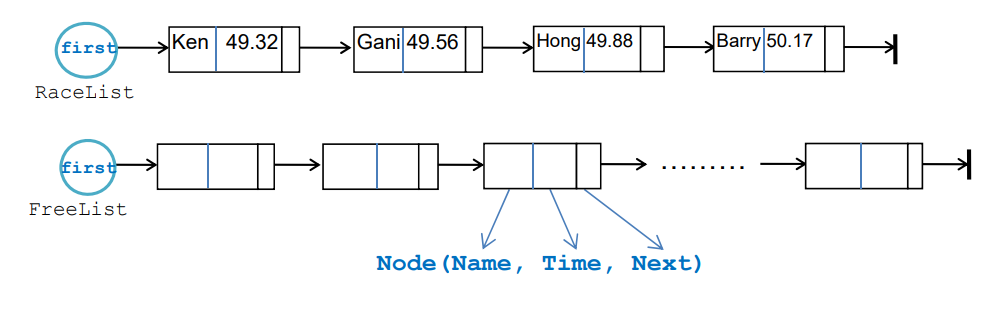
\includegraphics[width=0.65\paperwidth]{C:/Users/Admin/Desktop/Github/question_bank/LyX/static/img/9597-PJC-2014-P1-Q3}
\par\end{center}

\subsection*{Task 3.1 }

Write program code to create \texttt{Node} and \texttt{LinkedList},
and initialise an empty linked \texttt{RaceList}, and \texttt{FreeList}
of \textbf{20} nodes. Ensure all identifiers and methods specified
above are created. 

\subsection*{Evidence 8: }

Your program code for task 3.1. \hfill{}{[}17{]}

\subsection*{Evidence 9: }

Screenshot of running method to display \texttt{RaceList} and \texttt{FreeList}
on screen. \hfill{}{[}1{]}

\subsection*{Task 3.2 }

Write code to implement a method \texttt{AddInOrder} that will add
a new node with data into \texttt{RaceList} in ascending order of
running time. Node added to \texttt{RaceList} should be taken from
\texttt{FreeList}. 

\subsection*{Evidence 10: }

Your program code for task 3.2. \hfill{}{[}11{]}

\subsection*{Task 3.3 }

Test your program using the following data items input in the order
shown and run method to display \texttt{RaceList} and \texttt{FreeList}
on screen. 
\noindent \begin{center}
\begin{tabular}{|c|c|c|}
\hline 
\textbf{Order of input } & \textbf{Name} & \textbf{Running Time}\tabularnewline
\hline 
\hline 
1 & Barry & 50.17\tabularnewline
\hline 
2 & Gani  & 49.56\tabularnewline
\hline 
3 & Hong & 49.88\tabularnewline
\hline 
4 & Ken & 49.32 \tabularnewline
\hline 
\end{tabular} 
\par\end{center}

\subsection*{Evidence 11: }

Provide screenshot for task 3.3. \hfill{} {[}2{]}

\subsection*{Task 3.4 }

Write code to implement a method \texttt{RemoveNode} that will remove
the node that contains data specified by user to be removed from \texttt{RaceList}.
Node removed from \texttt{RaceList} should be returned to \texttt{FreeList}. 

\subsection*{Evidence 12: }

Your program code for task 3.4. \hfill{}{[}8{]}

\subsection*{Task 3.5 }

Test your program by removing \texttt{Gani} from \texttt{RaceList}
and run method to display \texttt{RaceL}ist and \texttt{FreeList}
on screen. 

\subsection*{Evidence 13: }

Provide screenshot for task 3.5. \hfill{} {[}1{]}

{[}SPLIT\_HERE{]}
\item \textbf{{[}PJC/PRELIM/9597/2014/P1/Q4{]} }

A message is encrypted and passed between two parties. To decrypt
the message, a \textquotedblleft key\textquotedblright{} is applied.
Both the sending and receiving parties hold the key which enables
them to encrypt and decrypt the message. 

An approach of cryptography is the simple substitution cipher, a method
of encryption by which each letter of a message is substituted with
another letter. The receiving party deciphers the text by performing
an inverse substitution. 

The substitution system is created by first writing out a \emph{phrase}.
The key is then derived from the phrase by removing all the repeated
letters. The \emph{cipher text} alphabet is then constructed starting
with the letters of the \emph{key} and then followed by all the remaining
letters in the alphabet. 

Using this system, the phrase \textquotedbl\texttt{apple}\textquotedbl{}
gives us the key as \textquotedbl\texttt{APLE}\textquotedbl{} and
the following substitution scheme: 

\begin{tabular}{cccccccccccccccccccccccccccc}
\textbf{Plain text alphabet :} & a & b & c & d & e & f & g & h & i & j & k & l & m & n & o & p & q & r & s & t & u & v & w & x & y & z & \tabularnewline
 & $\downarrow$ &  &  & $\downarrow$ & \multicolumn{21}{c}{$\cdots$$\cdots$$\cdots$$\cdots$$\cdots$$\cdots$$\cdots$$\cdots$} & $\downarrow$ & is substituted by\tabularnewline
\textbf{Cipher text alphabet :} & A & P & L & E & B & C & D & F & G & H & I & J & K & M & N & O & Q & R & S & T & U & V & W & X & Y & Z & \tabularnewline
\end{tabular}

\texttt{'a'} will be substituted by \texttt{'A'}, \texttt{'b'} will
be substituted by \texttt{'P'}, \texttt{'c'} will be substituted by
\texttt{'L'}, \texttt{'d'} will be substituted by\texttt{ 'E'},\texttt{
'e' }will be substituted by \texttt{'B'}, and so on. 

\subsection*{Task 4.1 }

Write program code for a function to create cipher text using the
following specification:
\noindent \begin{center}
\texttt{FUNCTION CreateCipher (phrase : STRING) : STRING }
\par\end{center}

The function \texttt{CreateCipher} has a single parameter \texttt{phrase}
and returns the cipher text alphabet as a string. 

\subsection*{Evidence 14: }

Your program code for task 4.1.\hfill{} {[}8{]}

\subsection*{Task 4.2 }

Write program code for a procedure \texttt{CreateCipherTest} which
does the following: 
\begin{itemize}
\item read the phrases from file phrases.txt 
\item create cipher text for each of the phrases 
\item display each phrase and cipher text on the screen as follows: 

\noindent\fbox{\begin{minipage}[t]{1\columnwidth - 2\fboxsep - 2\fboxrule}%
\texttt{Phrase: apple }

\texttt{Cipher text: APLEBCDFGHIJKMNOQRSTUVWXYZ }

\texttt{... ...}

\texttt{... ... }%
\end{minipage}}
\end{itemize}

\subsection*{Evidence 15: }

Your program code for task 4.2.\hfill{} {[}3{]}

\subsection*{Evidence 16: }

Screenshot for running task 4.2. \hfill{}{[}1{]}

\subsection*{Task 4.3}

Write program code for a function to decrypt a message using the following
specification: 
\noindent \begin{center}
\texttt{FUNCTION Decrypt (enc\_message:STRING, cipher:STRING) : STRING }
\par\end{center}

The function \texttt{Decrypt} accepts parameters \texttt{enc\_message}
and \texttt{cipher}, and returns the decrypted message as a string.
Parameter \texttt{enc\_message} is the encrypted message, and parameter
\texttt{cipher} is the cipher text alphabet. 

\subsection*{Evidence 17: }

Your program code for task 4.3. \hfill{}{[}6{]}

\subsection*{Task 4.4 }

Write program code which does the following: 
\begin{itemize}
\item read the phrase and encrypted message from file \texttt{cipher.txt }
\item cipher text is generated from \texttt{CreateCipher} function 
\item message is decrypted from \texttt{Decrypt} function 
\item display decrypted message on the screen together with the phrase and
encrypted message 

\noindent\fbox{\begin{minipage}[t]{1\columnwidth - 2\fboxsep - 2\fboxrule}%
\texttt{Phrase: ...}

\texttt{Encrypted message: ...}

\texttt{Decrypted message: ...}%
\end{minipage}}
\end{itemize}

\subsection*{Evidence 18: }

Your program code for task 4.4.\hfill{} {[}3{]}

\subsection*{Evidence 19: }

Screenshot for running task 4.4. \hfill{}{[}1{]}

\subsection*{Task 4.5 }

Write program code for a function to encrypt a message using the following
specification:

\texttt{FUNCTION Encrypt (message:STRING, cipher:STRING) : STRING}

The function \texttt{Encrypt} accepts parameters \texttt{message}
and \texttt{phrase}, and returns the encrypted message as a string.
Parameter \texttt{message} is the message to be encrypted while parameter
\texttt{cipher} is the cipher text. 

\subsection*{Evidence 20: }

Your program code for task 4.5.\hfill{} {[}4{]}

\subsection*{Task 4.6 }

Write program code which does the following: 
\begin{itemize}
\item encrypt the message: \textquotedblleft \texttt{do not give up!}\textquotedblright{}
\item use the phrase: \textquotedblleft \texttt{skyhigh}\textquotedblright{} 
\item generate cipher text from \texttt{CreateCipher} function
\item message is encrypted using \texttt{Encrypt} function
\item encrypted message is displayed on screen as follows: 

\noindent\fbox{\begin{minipage}[t]{1\columnwidth - 2\fboxsep - 2\fboxrule}%
\texttt{Phrase: skyhigh}

\texttt{Encrypted message: ...}%
\end{minipage}}
\end{itemize}

\subsection*{Evidence 21: }

Your program code for task 4.6. \hfill{}{[}3{]}

\subsection*{Evidence 22: }

Screenshot for running task 4.6. \hfill{}{[}1{]}

{[}SPLIT\_HERE{]}
\end{enumerate}

\end{document}
